 \documentclass[12pt]{article}
\usepackage[a4paper, margin=.30in]{geometry}

\usepackage{array}
\usepackage{graphicx, subfig, wrapfig, fancyhdr, lastpage }
\newcommand\headerMe[2]{\noindent{}#1\hfill#2}
\usepackage[mathscr]{euscript}



\pagestyle{fancy}
\fancyhf{}

\rfoot{\em{Page \thepage \hspace{1pt} / \pageref{LastPage}}}
\begin{document}

\headerMe{Royaume du Maroc}{année scolaire \emph{2022-2023}}\\
\headerMe{Ministère de l'Éducation nationale, }{  Professeur :\emph{Zakaria Haouzan}}\\
\headerMe{du Préscolaire et des Sports}{Établissement : \emph{Lycée SKHOR qualifiant}}\\

\begin{center}
Devoir  N°1-semestre 2 \\
   Filière Tronc Commun Scientifique\\
Durée 1h00
\\
    \vspace{.2cm}
\hrulefill
\Large{Chimie 7pts}
\hrulefill\\

    %\emph{Les Trois parties sont indépendantes}
\end{center}
%end Headerss------------------------
 \section*{Partie 1 :La quantité de matière \dotfill (7pts) }
La caféine, présente dans le café, le thé, le chocolat, les boissons au cola, est un stimulant pouvant être toxique à forte dose (plus de $600 mg$ par jour). Sa formule chimique est $C_8H_{10}N_4O_2$.

\begin{enumerate}
    \item Quelle est la masse molaire de la caféine?(avec M(N) = 14g/mol)\dotfill(1pt)
    \item Quelle quantité de matière de caféine y-a-t-il dans une tasse de café contenant 80 mg de caféine?\dotfill(1pt)
    \item Combien y-a-t-il de molécules de caféine dans la tasse?\dotfill(1pt)
    \item Combien de tasses de café peut-on boire par jour sans risque d’intoxication?\dotfill(2pt)
        \item Un café décaféiné en grains (ou moulu) ne doit pas contenir plus de 0,10 \% en masse de caféine.Quelle quantité de matière maximale de caféine y-a-t-il dans un paquet de café décaféiné de masse
            250g ?\dotfill(2pt)
\end{enumerate}
%__________________Chimie ______________________-
%%%%%%%+_+_+_+_+_+_+_+_+_Partie1

%_____________________________________PHYSIque Partie 22222____________________________________________________________________________
\begin{center}
    %\vspace{2cm}
\hrulefill
\Large{Physique 13pts}
\hrulefill\\
    %\emph{Les deux parties sont indépendantes}
\end{center}
%end Headerss------------------------

 \section*{Partie 1 :Equilibre d’un solide soumis à trois forces non parallèles et sans frottement \dotfill(7 pts)}
 \begin{wrapfigure}[4]{r}{0.3\textwidth}
	 \vspace{-1cm} 
    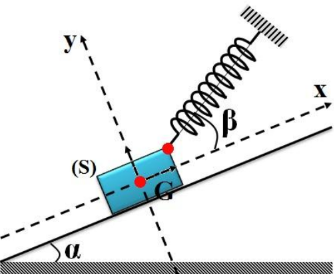
\includegraphics[width=0.3\textwidth]{./force_ing.png}
%\rule{3cm}{7cm}
\end{wrapfigure}
Un solide (S) de masse m = 200 g est maintenue à l’équilibre
sur un plan incliné parfaitement lisse d’inclinaison $\alpha= 30$° par
rapport à l’horizontale par l’intermédiaire d’un ressort de
masse négligeable, de constante de raideur $k = 40 N.m^{-1}$
et
allongé. L’axe du ressort fait un angle $\beta= 20$° avec la ligne de
la grande pente du plan incliné.
\begin{enumerate}
	\item  Rappeler la condition d’équilibre d’un solide soumis à trois
forces \\non parallèles.
\item  Faire l'inventaire des forces appliquées sur le solide (S) et
\\les représenter sur le schéma ci-contre.
\item  Ecrire la condition vectorielle d'équilibre du solide (S).
\item  Déterminer les expressions des coordonnées de ces forces dans le repère orthonormé .
\item  Exprimer l’allongement $\Delta{L}$ du ressort en fonction de m, g, $\alpha$, K et $\beta$. Calculer $\Delta{L}$.
\end{enumerate}

	Donnée: L'intensité de pesanteur: g = 10N/kg.


 \vspace{3cm}

\hrulefill\\
%_________________partie 2  : gravitation universelle :)
\section*{Partie 2 : Équilibre d'un corps solide en rotation autour d'un axe fixe\dotfill(6pts)}
Un homme maintient en équilibre un panneau de centre G, de
masse $m = 50kg$, et de longueur $OA = 2m$ dans une position
inclinée d’un angle $\alpha$ = 60° avec le sol. Il exerce en H, à la
distance $OH = 1,7m$ une force $\vec{F}$ perpendiculaire au panneau
comme indique la figure ci-contre. Le panneau peut tourner
autour de l’axe $(\Delta)$ passant par O

\begin{center}

    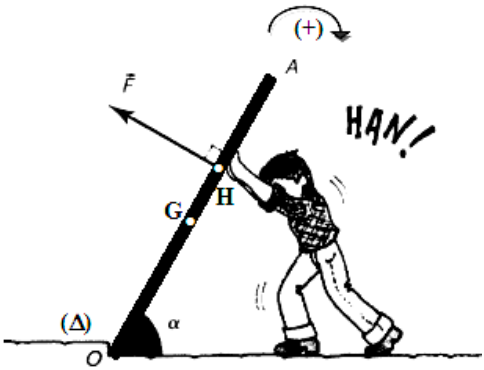
\includegraphics[width=0.36\textwidth]{./rotation.png}
\end{center}
\begin{enumerate}
    \item Faire l’inventaire des forces appliquées sur le panneau, et les
        représenter sur la figure.\dotfill(2pts)
    \item Enoncer le théorème des moments. \dotfill(1pt)
\item Trouver l’expression du moment de chaque force appliquée
    sur le panneau \dotfill(1pt)
\item En utilisant le théorème des moments, montrer que l’expression de l’intensité de la force $\vec{F}$ appliquée par l’homme s'écrit sous la forme :$$F = \frac{m.g.OA.cos\alpha}{2.OH}$$
    , et calculer sa valeur. \dotfill(2pts)
        \end{enumerate}



\end{document}
